\documentclass[twoside]{book}

% Packages required by doxygen
\usepackage{fixltx2e}
\usepackage{calc}
\usepackage{doxygen}
\usepackage[export]{adjustbox} % also loads graphicx
\usepackage{graphicx}
\usepackage[utf8]{inputenc}
\usepackage{makeidx}
\usepackage{multicol}
\usepackage{multirow}
\PassOptionsToPackage{warn}{textcomp}
\usepackage{textcomp}
\usepackage[nointegrals]{wasysym}
\usepackage[table]{xcolor}

% Font selection
\usepackage[T1]{fontenc}
\usepackage[scaled=.90]{helvet}
\usepackage{courier}
\usepackage{amssymb}
\usepackage{sectsty}
\renewcommand{\familydefault}{\sfdefault}
\allsectionsfont{%
  \fontseries{bc}\selectfont%
  \color{darkgray}%
}
\renewcommand{\DoxyLabelFont}{%
  \fontseries{bc}\selectfont%
  \color{darkgray}%
}
\newcommand{\+}{\discretionary{\mbox{\scriptsize$\hookleftarrow$}}{}{}}

% Page & text layout
\usepackage{geometry}
\geometry{%
  a4paper,%
  top=2.5cm,%
  bottom=2.5cm,%
  left=2.5cm,%
  right=2.5cm%
}
\tolerance=750
\hfuzz=15pt
\hbadness=750
\setlength{\emergencystretch}{15pt}
\setlength{\parindent}{0cm}
\setlength{\parskip}{3ex plus 2ex minus 2ex}
\makeatletter
\renewcommand{\paragraph}{%
  \@startsection{paragraph}{4}{0ex}{-1.0ex}{1.0ex}{%
    \normalfont\normalsize\bfseries\SS@parafont%
  }%
}
\renewcommand{\subparagraph}{%
  \@startsection{subparagraph}{5}{0ex}{-1.0ex}{1.0ex}{%
    \normalfont\normalsize\bfseries\SS@subparafont%
  }%
}
\makeatother

% Headers & footers
\usepackage{fancyhdr}
\pagestyle{fancyplain}
\fancyhead[LE]{\fancyplain{}{\bfseries\thepage}}
\fancyhead[CE]{\fancyplain{}{}}
\fancyhead[RE]{\fancyplain{}{\bfseries\leftmark}}
\fancyhead[LO]{\fancyplain{}{\bfseries\rightmark}}
\fancyhead[CO]{\fancyplain{}{}}
\fancyhead[RO]{\fancyplain{}{\bfseries\thepage}}
\fancyfoot[LE]{\fancyplain{}{}}
\fancyfoot[CE]{\fancyplain{}{}}
\fancyfoot[RE]{\fancyplain{}{\bfseries\scriptsize Generated by Doxygen }}
\fancyfoot[LO]{\fancyplain{}{\bfseries\scriptsize Generated by Doxygen }}
\fancyfoot[CO]{\fancyplain{}{}}
\fancyfoot[RO]{\fancyplain{}{}}
\renewcommand{\footrulewidth}{0.4pt}
\renewcommand{\chaptermark}[1]{%
  \markboth{#1}{}%
}
\renewcommand{\sectionmark}[1]{%
  \markright{\thesection\ #1}%
}

% Indices & bibliography
\usepackage{natbib}
\usepackage[titles]{tocloft}
\setcounter{tocdepth}{3}
\setcounter{secnumdepth}{5}
\makeindex

% Hyperlinks (required, but should be loaded last)
\usepackage{ifpdf}
\ifpdf
  \usepackage[pdftex,pagebackref=true]{hyperref}
\else
  \usepackage[ps2pdf,pagebackref=true]{hyperref}
\fi
\hypersetup{%
  colorlinks=true,%
  linkcolor=blue,%
  citecolor=blue,%
  unicode%
}

% Custom commands
\newcommand{\clearemptydoublepage}{%
  \newpage{\pagestyle{empty}\cleardoublepage}%
}

\usepackage{caption}
\captionsetup{labelsep=space,justification=centering,font={bf},singlelinecheck=off,skip=4pt,position=top}

%===== C O N T E N T S =====

\begin{document}

% Titlepage & ToC
\hypersetup{pageanchor=false,
             bookmarksnumbered=true,
             pdfencoding=unicode
            }
\pagenumbering{roman}
\begin{titlepage}
\vspace*{7cm}
\begin{center}%
{\Large P\+A09 }\\
\vspace*{1cm}
{\large Generated by Doxygen 1.8.11}\\
\end{center}
\end{titlepage}
\clearemptydoublepage
\tableofcontents
\clearemptydoublepage
\pagenumbering{arabic}
\hypersetup{pageanchor=true}

%--- Begin generated contents ---
\chapter{Hierarchical Index}
\section{Class Hierarchy}
This inheritance list is sorted roughly, but not completely, alphabetically\+:\begin{DoxyCompactList}
\item \contentsline{section}{Greater$<$ Key\+Type $>$}{\pageref{class_greater}}{}
\item \contentsline{section}{Heap$<$ Data\+Type, Key\+Type, Comparator $>$}{\pageref{class_heap}}{}
\item \contentsline{section}{Heap$<$ Data\+Type $>$}{\pageref{class_heap}}{}
\begin{DoxyCompactList}
\item \contentsline{section}{Priority\+Queue$<$ Data\+Type, Key\+Type, Comparator $>$}{\pageref{class_priority_queue}}{}
\end{DoxyCompactList}
\item \contentsline{section}{Less$<$ Key\+Type $>$}{\pageref{class_less}}{}
\item \contentsline{section}{Less$<$ int $>$}{\pageref{class_less}}{}
\item \contentsline{section}{Task\+Data}{\pageref{struct_task_data}}{}
\item \contentsline{section}{Test\+Data}{\pageref{class_test_data}}{}
\item \contentsline{section}{Test\+Data\+Item$<$ Key\+Type $>$}{\pageref{class_test_data_item}}{}
\end{DoxyCompactList}

\chapter{Class Index}
\section{Class List}
Here are the classes, structs, unions and interfaces with brief descriptions\+:\begin{DoxyCompactList}
\item\contentsline{section}{\hyperlink{class_board}{Board} }{\pageref{class_board}}{}
\item\contentsline{section}{\hyperlink{classrush_board}{rush\+Board} }{\pageref{classrush_board}}{}
\item\contentsline{section}{\hyperlink{struct_vehicle}{Vehicle} }{\pageref{struct_vehicle}}{}
\end{DoxyCompactList}

\chapter{File Index}
\section{File List}
Here is a list of all files with brief descriptions\+:\begin{DoxyCompactList}
\item\contentsline{section}{\hyperlink{_hash_table_8cpp}{Hash\+Table.\+cpp} \\*An implementation file for a \hyperlink{class_hash_table}{Hash\+Table} }{\pageref{_hash_table_8cpp}}{}
\item\contentsline{section}{\hyperlink{_hash_table_8h}{Hash\+Table.\+h} }{\pageref{_hash_table_8h}}{}
\item\contentsline{section}{\hyperlink{login_8cpp}{login.\+cpp} \\*Programming Exercise \#1 for a Hash Table }{\pageref{login_8cpp}}{}
\end{DoxyCompactList}

\chapter{Class Documentation}
\hypertarget{class_greater}{}\section{Greater$<$ Key\+Type $>$ Class Template Reference}
\label{class_greater}\index{Greater$<$ Key\+Type $>$@{Greater$<$ Key\+Type $>$}}
\subsection*{Public Member Functions}
\begin{DoxyCompactItemize}
\item 
bool \hyperlink{class_greater_a79d9cb7121723ee9d65b11cb2fce0379}{operator()} (const Key\+Type \&a, const Key\+Type \&b) const 
\end{DoxyCompactItemize}


\subsection{Member Function Documentation}
\index{Greater@{Greater}!operator()@{operator()}}
\index{operator()@{operator()}!Greater@{Greater}}
\subsubsection[{\texorpdfstring{operator()(const Key\+Type \&a, const Key\+Type \&b) const }{operator()(const KeyType &a, const KeyType &b) const }}]{\setlength{\rightskip}{0pt plus 5cm}template$<$typename Key\+Type  = int$>$ bool {\bf Greater}$<$ Key\+Type $>$\+::operator() (
\begin{DoxyParamCaption}
\item[{const Key\+Type \&}]{a, }
\item[{const Key\+Type \&}]{b}
\end{DoxyParamCaption}
) const\hspace{0.3cm}{\ttfamily [inline]}}\hypertarget{class_greater_a79d9cb7121723ee9d65b11cb2fce0379}{}\label{class_greater_a79d9cb7121723ee9d65b11cb2fce0379}


The documentation for this class was generated from the following file\+:\begin{DoxyCompactItemize}
\item 
\hyperlink{test11_8cpp}{test11.\+cpp}\end{DoxyCompactItemize}

\hypertarget{class_heap}{}\section{Heap$<$ Data\+Type, Key\+Type, Comparator $>$ Class Template Reference}
\label{class_heap}\index{Heap$<$ Data\+Type, Key\+Type, Comparator $>$@{Heap$<$ Data\+Type, Key\+Type, Comparator $>$}}


{\ttfamily \#include $<$Heap.\+h$>$}

\subsection*{Public Member Functions}
\begin{DoxyCompactItemize}
\item 
\hyperlink{class_heap_ae17e34e3c86d88263a8fdf80b9ba78fc}{Heap} (int max\+Number=\hyperlink{class_heap_a967c19732a20a72e8e824402ad6763c8}{D\+E\+F\+A\+U\+L\+T\+\_\+\+M\+A\+X\+\_\+\+H\+E\+A\+P\+\_\+\+S\+I\+ZE})
\begin{DoxyCompactList}\small\item\em \char`\"{}\+Constructor. Creates an empty heap. Allocates enoughy memory for a heap containing max\+Number data items.\char`\"{} \end{DoxyCompactList}\item 
\hyperlink{class_heap_a97e3b462be1c6af31d7519546bba8907}{Heap} (const \hyperlink{class_heap}{Heap} \&other)
\begin{DoxyCompactList}\small\item\em \char`\"{}\+Copy constructor. Initializes the object to be an equivalent copy of other.\char`\"{} \end{DoxyCompactList}\item 
\hyperlink{class_heap}{Heap} \& \hyperlink{class_heap_a5ed119341c39bcea1437321d4247dd40}{operator=} (const \hyperlink{class_heap}{Heap} \&other)
\begin{DoxyCompactList}\small\item\em \char`\"{}\+Overloaded assignment operator. Sets the heap to be equivalent to the other Heap and returns a reference to this object.\char`\"{} \end{DoxyCompactList}\item 
\hyperlink{class_heap_a555ade7891007de959bef0ee53e28767}{$\sim$\+Heap} ()
\begin{DoxyCompactList}\small\item\em \char`\"{}\+Destructor. Deallocates (free) the memory used to store the heap.\char`\"{} \end{DoxyCompactList}\item 
void \hyperlink{class_heap_aa68cf80454ab1b246fa723612805a91e}{insert} (const Data\+Type \&new\+Data\+Item)  throw ( logic\+\_\+error )
\begin{DoxyCompactList}\small\item\em \char`\"{}\+Inserts new\+Data\+Item into the heap. Inserts this data item as the bottom rightmost data item in the heap and moves it upward until the properties that define a heap are restored.\char`\"{} \end{DoxyCompactList}\item 
Data\+Type \hyperlink{class_heap_a4a18bfdacd897c45fc3da13f22b8930d}{remove} ()  throw ( logic\+\_\+error )
\begin{DoxyCompactList}\small\item\em \char`\"{}\+Removes the data item with the highest priority (the root) from the heap and returns it. Replaces the root data item with the bottom rightmost data item and moves this data item downward until the properties that define a heap are restored.\char`\"{} \end{DoxyCompactList}\item 
void \hyperlink{class_heap_a19a78c8eae2cf7c8253e34e54d86ed73}{clear} ()
\begin{DoxyCompactList}\small\item\em \char`\"{}\+Removes all the data items in the heap.\char`\"{} \end{DoxyCompactList}\item 
bool \hyperlink{class_heap_ab8fa26d416ac0e27dfcbf18c54f8f73f}{is\+Empty} () const 
\begin{DoxyCompactList}\small\item\em \char`\"{}\+Returns true if the heap is empty. Otherwise, returns false.\char`\"{} \end{DoxyCompactList}\item 
bool \hyperlink{class_heap_ac9111b884c74a376240e0155a788756e}{is\+Full} () const 
\begin{DoxyCompactList}\small\item\em \char`\"{}\+Returns true if the heap is full. Otherwise, returns false.\char`\"{} \end{DoxyCompactList}\item 
void \hyperlink{class_heap_a3ae1e1f27a145749c8b9f2da777cb8bc}{show\+Structure} () const 
\item 
void \hyperlink{class_heap_a4bdb1772ea92899de245d6cbd217d085}{write\+Levels} () const 
\begin{DoxyCompactList}\small\item\em \char`\"{}\+Outputs the data items in a heap in level order, one level per line. Only outputs each data item\textquotesingle{}s priority. If the heap is empty, then outputs \textquotesingle{}\+Empty heap\textquotesingle{}.\char`\"{} \end{DoxyCompactList}\item 
int \hyperlink{class_heap_a35ffb267d73fdd5c106f82459b69cf2f}{get\+Left\+Child} (const int node\+Index) const 
\begin{DoxyCompactList}\small\item\em returns the left child \end{DoxyCompactList}\item 
int \hyperlink{class_heap_ae367797460e0f8923b72c1379ec9a9c2}{get\+Right\+Child} (const int node\+Index) const 
\begin{DoxyCompactList}\small\item\em returns the right child \end{DoxyCompactList}\item 
int \hyperlink{class_heap_a524cd0cd256e21b565f04b26297c0fd8}{get\+Parent} (const int node\+Index) const 
\begin{DoxyCompactList}\small\item\em returns the parent \end{DoxyCompactList}\item 
void \hyperlink{class_heap_a08cf707b0057b977fc1896bf38800027}{sort\+Up} (const int node\+Index)
\begin{DoxyCompactList}\small\item\em The sort\+Up function that recursively sorts for \hyperlink{class_heap_aa68cf80454ab1b246fa723612805a91e}{insert()} \end{DoxyCompactList}\item 
void \hyperlink{class_heap_a31eaa08f4ad1159b6272e0e32486702c}{sort\+Down} (const int node\+Index)
\begin{DoxyCompactList}\small\item\em The sort\+Down function that recursively sorts for \hyperlink{class_heap_a4a18bfdacd897c45fc3da13f22b8930d}{remove()} \end{DoxyCompactList}\end{DoxyCompactItemize}
\subsection*{Static Public Attributes}
\begin{DoxyCompactItemize}
\item 
static const int \hyperlink{class_heap_a967c19732a20a72e8e824402ad6763c8}{D\+E\+F\+A\+U\+L\+T\+\_\+\+M\+A\+X\+\_\+\+H\+E\+A\+P\+\_\+\+S\+I\+ZE} = 10
\end{DoxyCompactItemize}


\subsection{Constructor \& Destructor Documentation}
\index{Heap@{Heap}!Heap@{Heap}}
\index{Heap@{Heap}!Heap@{Heap}}
\subsubsection[{\texorpdfstring{Heap(int max\+Number=\+D\+E\+F\+A\+U\+L\+T\+\_\+\+M\+A\+X\+\_\+\+H\+E\+A\+P\+\_\+\+S\+I\+Z\+E)}{Heap(int maxNumber=DEFAULT_MAX_HEAP_SIZE)}}]{\setlength{\rightskip}{0pt plus 5cm}template$<$typename Data\+Type , typename Key\+Type , typename Comparator $>$ {\bf Heap}$<$ Data\+Type, Key\+Type, Comparator $>$\+::{\bf Heap} (
\begin{DoxyParamCaption}
\item[{int}]{max\+Number = {\ttfamily {\bf D\+E\+F\+A\+U\+L\+T\+\_\+\+M\+A\+X\+\_\+\+H\+E\+A\+P\+\_\+\+S\+I\+ZE}}}
\end{DoxyParamCaption}
)}\hypertarget{class_heap_ae17e34e3c86d88263a8fdf80b9ba78fc}{}\label{class_heap_ae17e34e3c86d88263a8fdf80b9ba78fc}


\char`\"{}\+Constructor. Creates an empty heap. Allocates enoughy memory for a heap containing max\+Number data items.\char`\"{} 


\begin{DoxyParams}{Parameters}
{\em int} & max\+Number \\
\hline
\end{DoxyParams}
\begin{DoxyReturn}{Returns}
none 
\end{DoxyReturn}
\index{Heap@{Heap}!Heap@{Heap}}
\index{Heap@{Heap}!Heap@{Heap}}
\subsubsection[{\texorpdfstring{Heap(const Heap \&other)}{Heap(const Heap &other)}}]{\setlength{\rightskip}{0pt plus 5cm}template$<$typename Data\+Type , typename Key\+Type , typename Comparator $>$ {\bf Heap}$<$ Data\+Type, Key\+Type, Comparator $>$\+::{\bf Heap} (
\begin{DoxyParamCaption}
\item[{const {\bf Heap}$<$ Data\+Type, Key\+Type, Comparator $>$ \&}]{other}
\end{DoxyParamCaption}
)}\hypertarget{class_heap_a97e3b462be1c6af31d7519546bba8907}{}\label{class_heap_a97e3b462be1c6af31d7519546bba8907}


\char`\"{}\+Copy constructor. Initializes the object to be an equivalent copy of other.\char`\"{} 


\begin{DoxyParams}{Parameters}
{\em const} & \hyperlink{class_heap}{Heap}\& other \\
\hline
\end{DoxyParams}
\begin{DoxyReturn}{Returns}
none 
\end{DoxyReturn}
\index{Heap@{Heap}!````~Heap@{$\sim$\+Heap}}
\index{````~Heap@{$\sim$\+Heap}!Heap@{Heap}}
\subsubsection[{\texorpdfstring{$\sim$\+Heap()}{~Heap()}}]{\setlength{\rightskip}{0pt plus 5cm}template$<$typename Data\+Type , typename Key\+Type , typename Comparator $>$ {\bf Heap}$<$ Data\+Type, Key\+Type, Comparator $>$\+::$\sim${\bf Heap} (
\begin{DoxyParamCaption}
{}
\end{DoxyParamCaption}
)}\hypertarget{class_heap_a555ade7891007de959bef0ee53e28767}{}\label{class_heap_a555ade7891007de959bef0ee53e28767}


\char`\"{}\+Destructor. Deallocates (free) the memory used to store the heap.\char`\"{} 


\begin{DoxyParams}{Parameters}
{\em none} & \\
\hline
\end{DoxyParams}
\begin{DoxyReturn}{Returns}
none 
\end{DoxyReturn}


\subsection{Member Function Documentation}
\index{Heap@{Heap}!clear@{clear}}
\index{clear@{clear}!Heap@{Heap}}
\subsubsection[{\texorpdfstring{clear()}{clear()}}]{\setlength{\rightskip}{0pt plus 5cm}template$<$typename Data\+Type , typename Key\+Type , typename Comparator $>$ void {\bf Heap}$<$ Data\+Type, Key\+Type, Comparator $>$\+::clear (
\begin{DoxyParamCaption}
{}
\end{DoxyParamCaption}
)}\hypertarget{class_heap_a19a78c8eae2cf7c8253e34e54d86ed73}{}\label{class_heap_a19a78c8eae2cf7c8253e34e54d86ed73}


\char`\"{}\+Removes all the data items in the heap.\char`\"{} 


\begin{DoxyParams}{Parameters}
{\em none} & \\
\hline
\end{DoxyParams}
\begin{DoxyReturn}{Returns}
none 
\end{DoxyReturn}
\index{Heap@{Heap}!get\+Left\+Child@{get\+Left\+Child}}
\index{get\+Left\+Child@{get\+Left\+Child}!Heap@{Heap}}
\subsubsection[{\texorpdfstring{get\+Left\+Child(const int node\+Index) const }{getLeftChild(const int nodeIndex) const }}]{\setlength{\rightskip}{0pt plus 5cm}template$<$typename Data\+Type , typename Key\+Type , typename Comparator $>$ int {\bf Heap}$<$ Data\+Type, Key\+Type, Comparator $>$\+::get\+Left\+Child (
\begin{DoxyParamCaption}
\item[{const int}]{node\+Index}
\end{DoxyParamCaption}
) const}\hypertarget{class_heap_a35ffb267d73fdd5c106f82459b69cf2f}{}\label{class_heap_a35ffb267d73fdd5c106f82459b69cf2f}


returns the left child 


\begin{DoxyParams}{Parameters}
{\em const} & int node\+Index \\
\hline
\end{DoxyParams}
\begin{DoxyReturn}{Returns}
(2 $\ast$ node\+Index + 1) 
\end{DoxyReturn}
\index{Heap@{Heap}!get\+Parent@{get\+Parent}}
\index{get\+Parent@{get\+Parent}!Heap@{Heap}}
\subsubsection[{\texorpdfstring{get\+Parent(const int node\+Index) const }{getParent(const int nodeIndex) const }}]{\setlength{\rightskip}{0pt plus 5cm}template$<$typename Data\+Type , typename Key\+Type , typename Comparator $>$ int {\bf Heap}$<$ Data\+Type, Key\+Type, Comparator $>$\+::get\+Parent (
\begin{DoxyParamCaption}
\item[{const int}]{node\+Index}
\end{DoxyParamCaption}
) const}\hypertarget{class_heap_a524cd0cd256e21b565f04b26297c0fd8}{}\label{class_heap_a524cd0cd256e21b565f04b26297c0fd8}


returns the parent 


\begin{DoxyParams}{Parameters}
{\em const} & int node\+Index \\
\hline
\end{DoxyParams}
\begin{DoxyReturn}{Returns}
(node\+Index / 2) -\/ 1 or (node\+Index / 2) 
\end{DoxyReturn}
\index{Heap@{Heap}!get\+Right\+Child@{get\+Right\+Child}}
\index{get\+Right\+Child@{get\+Right\+Child}!Heap@{Heap}}
\subsubsection[{\texorpdfstring{get\+Right\+Child(const int node\+Index) const }{getRightChild(const int nodeIndex) const }}]{\setlength{\rightskip}{0pt plus 5cm}template$<$typename Data\+Type , typename Key\+Type , typename Comparator $>$ int {\bf Heap}$<$ Data\+Type, Key\+Type, Comparator $>$\+::get\+Right\+Child (
\begin{DoxyParamCaption}
\item[{const int}]{node\+Index}
\end{DoxyParamCaption}
) const}\hypertarget{class_heap_ae367797460e0f8923b72c1379ec9a9c2}{}\label{class_heap_ae367797460e0f8923b72c1379ec9a9c2}


returns the right child 


\begin{DoxyParams}{Parameters}
{\em const} & int node\+Index \\
\hline
\end{DoxyParams}
\begin{DoxyReturn}{Returns}
(2 $\ast$ node\+Index + 2) 
\end{DoxyReturn}
\index{Heap@{Heap}!insert@{insert}}
\index{insert@{insert}!Heap@{Heap}}
\subsubsection[{\texorpdfstring{insert(const Data\+Type \&new\+Data\+Item)}{insert(const DataType &newDataItem)}}]{\setlength{\rightskip}{0pt plus 5cm}template$<$typename Data\+Type, typename Key\+Type , typename Comparator $>$ void {\bf Heap}$<$ Data\+Type, Key\+Type, Comparator $>$\+::insert (
\begin{DoxyParamCaption}
\item[{const Data\+Type \&}]{new\+Data\+Item}
\end{DoxyParamCaption}
) throw  logic\+\_\+error) }\hypertarget{class_heap_aa68cf80454ab1b246fa723612805a91e}{}\label{class_heap_aa68cf80454ab1b246fa723612805a91e}


\char`\"{}\+Inserts new\+Data\+Item into the heap. Inserts this data item as the bottom rightmost data item in the heap and moves it upward until the properties that define a heap are restored.\char`\"{} 


\begin{DoxyParams}{Parameters}
{\em const} & Data\+Type\& new\+Data\+Item \\
\hline
\end{DoxyParams}
\begin{DoxyReturn}{Returns}
none 
\end{DoxyReturn}
\index{Heap@{Heap}!is\+Empty@{is\+Empty}}
\index{is\+Empty@{is\+Empty}!Heap@{Heap}}
\subsubsection[{\texorpdfstring{is\+Empty() const }{isEmpty() const }}]{\setlength{\rightskip}{0pt plus 5cm}template$<$typename Data\+Type , typename Key\+Type , typename Comparator $>$ bool {\bf Heap}$<$ Data\+Type, Key\+Type, Comparator $>$\+::is\+Empty (
\begin{DoxyParamCaption}
{}
\end{DoxyParamCaption}
) const}\hypertarget{class_heap_ab8fa26d416ac0e27dfcbf18c54f8f73f}{}\label{class_heap_ab8fa26d416ac0e27dfcbf18c54f8f73f}


\char`\"{}\+Returns true if the heap is empty. Otherwise, returns false.\char`\"{} 


\begin{DoxyParams}{Parameters}
{\em none} & \\
\hline
\end{DoxyParams}
\begin{DoxyReturn}{Returns}
true or false 
\end{DoxyReturn}
\index{Heap@{Heap}!is\+Full@{is\+Full}}
\index{is\+Full@{is\+Full}!Heap@{Heap}}
\subsubsection[{\texorpdfstring{is\+Full() const }{isFull() const }}]{\setlength{\rightskip}{0pt plus 5cm}template$<$typename Data\+Type , typename Key\+Type , typename Comparator $>$ bool {\bf Heap}$<$ Data\+Type, Key\+Type, Comparator $>$\+::is\+Full (
\begin{DoxyParamCaption}
{}
\end{DoxyParamCaption}
) const}\hypertarget{class_heap_ac9111b884c74a376240e0155a788756e}{}\label{class_heap_ac9111b884c74a376240e0155a788756e}


\char`\"{}\+Returns true if the heap is full. Otherwise, returns false.\char`\"{} 


\begin{DoxyParams}{Parameters}
{\em none} & \\
\hline
\end{DoxyParams}
\begin{DoxyReturn}{Returns}
true or false 
\end{DoxyReturn}
\index{Heap@{Heap}!operator=@{operator=}}
\index{operator=@{operator=}!Heap@{Heap}}
\subsubsection[{\texorpdfstring{operator=(const Heap \&other)}{operator=(const Heap &other)}}]{\setlength{\rightskip}{0pt plus 5cm}template$<$typename Data\+Type , typename Key\+Type , typename Comparator $>$ {\bf Heap}$<$ Data\+Type, Key\+Type, Comparator $>$ \& {\bf Heap}$<$ Data\+Type, Key\+Type, Comparator $>$\+::operator= (
\begin{DoxyParamCaption}
\item[{const {\bf Heap}$<$ Data\+Type, Key\+Type, Comparator $>$ \&}]{other}
\end{DoxyParamCaption}
)}\hypertarget{class_heap_a5ed119341c39bcea1437321d4247dd40}{}\label{class_heap_a5ed119341c39bcea1437321d4247dd40}


\char`\"{}\+Overloaded assignment operator. Sets the heap to be equivalent to the other Heap and returns a reference to this object.\char`\"{} 


\begin{DoxyParams}{Parameters}
{\em const} & \hyperlink{class_heap}{Heap}\& other \\
\hline
\end{DoxyParams}
\begin{DoxyReturn}{Returns}
$\ast$this 
\end{DoxyReturn}
\index{Heap@{Heap}!remove@{remove}}
\index{remove@{remove}!Heap@{Heap}}
\subsubsection[{\texorpdfstring{remove()}{remove()}}]{\setlength{\rightskip}{0pt plus 5cm}template$<$typename Data\+Type , typename Key\+Type , typename Comparator $>$ Data\+Type {\bf Heap}$<$ Data\+Type, Key\+Type, Comparator $>$\+::remove (
\begin{DoxyParamCaption}
{}
\end{DoxyParamCaption}
) throw  logic\+\_\+error) }\hypertarget{class_heap_a4a18bfdacd897c45fc3da13f22b8930d}{}\label{class_heap_a4a18bfdacd897c45fc3da13f22b8930d}


\char`\"{}\+Removes the data item with the highest priority (the root) from the heap and returns it. Replaces the root data item with the bottom rightmost data item and moves this data item downward until the properties that define a heap are restored.\char`\"{} 


\begin{DoxyParams}{Parameters}
{\em none} & \\
\hline
\end{DoxyParams}
\begin{DoxyReturn}{Returns}
Datatype temp 
\end{DoxyReturn}
\index{Heap@{Heap}!show\+Structure@{show\+Structure}}
\index{show\+Structure@{show\+Structure}!Heap@{Heap}}
\subsubsection[{\texorpdfstring{show\+Structure() const }{showStructure() const }}]{\setlength{\rightskip}{0pt plus 5cm}template$<$typename Data\+Type , typename Key\+Type , typename Comparator $>$ void {\bf Heap}$<$ Data\+Type, Key\+Type, Comparator $>$\+::show\+Structure (
\begin{DoxyParamCaption}
{}
\end{DoxyParamCaption}
) const}\hypertarget{class_heap_a3ae1e1f27a145749c8b9f2da777cb8bc}{}\label{class_heap_a3ae1e1f27a145749c8b9f2da777cb8bc}
\index{Heap@{Heap}!sort\+Down@{sort\+Down}}
\index{sort\+Down@{sort\+Down}!Heap@{Heap}}
\subsubsection[{\texorpdfstring{sort\+Down(const int node\+Index)}{sortDown(const int nodeIndex)}}]{\setlength{\rightskip}{0pt plus 5cm}template$<$typename Data\+Type , typename Key\+Type , typename Comparator $>$ void {\bf Heap}$<$ Data\+Type, Key\+Type, Comparator $>$\+::sort\+Down (
\begin{DoxyParamCaption}
\item[{const int}]{node\+Index}
\end{DoxyParamCaption}
)}\hypertarget{class_heap_a31eaa08f4ad1159b6272e0e32486702c}{}\label{class_heap_a31eaa08f4ad1159b6272e0e32486702c}


The sort\+Down function that recursively sorts for \hyperlink{class_heap_a4a18bfdacd897c45fc3da13f22b8930d}{remove()} 


\begin{DoxyParams}{Parameters}
{\em const} & int node\+Index \\
\hline
\end{DoxyParams}
\begin{DoxyReturn}{Returns}
none 
\end{DoxyReturn}
\index{Heap@{Heap}!sort\+Up@{sort\+Up}}
\index{sort\+Up@{sort\+Up}!Heap@{Heap}}
\subsubsection[{\texorpdfstring{sort\+Up(const int node\+Index)}{sortUp(const int nodeIndex)}}]{\setlength{\rightskip}{0pt plus 5cm}template$<$typename Data\+Type , typename Key\+Type , typename Comparator $>$ void {\bf Heap}$<$ Data\+Type, Key\+Type, Comparator $>$\+::sort\+Up (
\begin{DoxyParamCaption}
\item[{const int}]{node\+Index}
\end{DoxyParamCaption}
)}\hypertarget{class_heap_a08cf707b0057b977fc1896bf38800027}{}\label{class_heap_a08cf707b0057b977fc1896bf38800027}


The sort\+Up function that recursively sorts for \hyperlink{class_heap_aa68cf80454ab1b246fa723612805a91e}{insert()} 


\begin{DoxyParams}{Parameters}
{\em const} & int node\+Index \\
\hline
\end{DoxyParams}
\begin{DoxyReturn}{Returns}
none 
\end{DoxyReturn}
\index{Heap@{Heap}!write\+Levels@{write\+Levels}}
\index{write\+Levels@{write\+Levels}!Heap@{Heap}}
\subsubsection[{\texorpdfstring{write\+Levels() const }{writeLevels() const }}]{\setlength{\rightskip}{0pt plus 5cm}template$<$typename Data\+Type , typename Key\+Type , typename Comparator $>$ void {\bf Heap}$<$ Data\+Type, Key\+Type, Comparator $>$\+::write\+Levels (
\begin{DoxyParamCaption}
{}
\end{DoxyParamCaption}
) const}\hypertarget{class_heap_a4bdb1772ea92899de245d6cbd217d085}{}\label{class_heap_a4bdb1772ea92899de245d6cbd217d085}


\char`\"{}\+Outputs the data items in a heap in level order, one level per line. Only outputs each data item\textquotesingle{}s priority. If the heap is empty, then outputs \textquotesingle{}\+Empty heap\textquotesingle{}.\char`\"{} 


\begin{DoxyParams}{Parameters}
{\em none} & \\
\hline
\end{DoxyParams}
\begin{DoxyReturn}{Returns}
none 
\end{DoxyReturn}


\subsection{Member Data Documentation}
\index{Heap@{Heap}!D\+E\+F\+A\+U\+L\+T\+\_\+\+M\+A\+X\+\_\+\+H\+E\+A\+P\+\_\+\+S\+I\+ZE@{D\+E\+F\+A\+U\+L\+T\+\_\+\+M\+A\+X\+\_\+\+H\+E\+A\+P\+\_\+\+S\+I\+ZE}}
\index{D\+E\+F\+A\+U\+L\+T\+\_\+\+M\+A\+X\+\_\+\+H\+E\+A\+P\+\_\+\+S\+I\+ZE@{D\+E\+F\+A\+U\+L\+T\+\_\+\+M\+A\+X\+\_\+\+H\+E\+A\+P\+\_\+\+S\+I\+ZE}!Heap@{Heap}}
\subsubsection[{\texorpdfstring{D\+E\+F\+A\+U\+L\+T\+\_\+\+M\+A\+X\+\_\+\+H\+E\+A\+P\+\_\+\+S\+I\+ZE}{DEFAULT_MAX_HEAP_SIZE}}]{\setlength{\rightskip}{0pt plus 5cm}template$<$typename Data\+Type, typename Key\+Type = int, typename Comparator = Less$<$\+Key\+Type$>$$>$ const int {\bf Heap}$<$ Data\+Type, Key\+Type, Comparator $>$\+::D\+E\+F\+A\+U\+L\+T\+\_\+\+M\+A\+X\+\_\+\+H\+E\+A\+P\+\_\+\+S\+I\+ZE = 10\hspace{0.3cm}{\ttfamily [static]}}\hypertarget{class_heap_a967c19732a20a72e8e824402ad6763c8}{}\label{class_heap_a967c19732a20a72e8e824402ad6763c8}


The documentation for this class was generated from the following files\+:\begin{DoxyCompactItemize}
\item 
\hyperlink{_heap_8h}{Heap.\+h}\item 
\hyperlink{_heap_8cpp}{Heap.\+cpp}\item 
\hyperlink{show11_8cpp}{show11.\+cpp}\end{DoxyCompactItemize}

\hypertarget{class_less}{}\section{Less$<$ Key\+Type $>$ Class Template Reference}
\label{class_less}\index{Less$<$ Key\+Type $>$@{Less$<$ Key\+Type $>$}}


{\ttfamily \#include $<$Heap.\+h$>$}

\subsection*{Public Member Functions}
\begin{DoxyCompactItemize}
\item 
bool \hyperlink{class_less_afee76a5248eb9c6c8fd1f005360d44d5}{operator()} (const Key\+Type \&a, const Key\+Type \&b) const 
\end{DoxyCompactItemize}


\subsection{Member Function Documentation}
\index{Less@{Less}!operator()@{operator()}}
\index{operator()@{operator()}!Less@{Less}}
\subsubsection[{\texorpdfstring{operator()(const Key\+Type \&a, const Key\+Type \&b) const }{operator()(const KeyType &a, const KeyType &b) const }}]{\setlength{\rightskip}{0pt plus 5cm}template$<$typename Key\+Type = int$>$ bool {\bf Less}$<$ Key\+Type $>$\+::operator() (
\begin{DoxyParamCaption}
\item[{const Key\+Type \&}]{a, }
\item[{const Key\+Type \&}]{b}
\end{DoxyParamCaption}
) const\hspace{0.3cm}{\ttfamily [inline]}}\hypertarget{class_less_afee76a5248eb9c6c8fd1f005360d44d5}{}\label{class_less_afee76a5248eb9c6c8fd1f005360d44d5}


The documentation for this class was generated from the following file\+:\begin{DoxyCompactItemize}
\item 
\hyperlink{_heap_8h}{Heap.\+h}\end{DoxyCompactItemize}

\hypertarget{class_priority_queue}{}\section{Priority\+Queue$<$ Data\+Type, Key\+Type, Comparator $>$ Class Template Reference}
\label{class_priority_queue}\index{Priority\+Queue$<$ Data\+Type, Key\+Type, Comparator $>$@{Priority\+Queue$<$ Data\+Type, Key\+Type, Comparator $>$}}


{\ttfamily \#include $<$Priority\+Queue.\+h$>$}

Inheritance diagram for Priority\+Queue$<$ Data\+Type, Key\+Type, Comparator $>$\+:\begin{figure}[H]
\begin{center}
\leavevmode
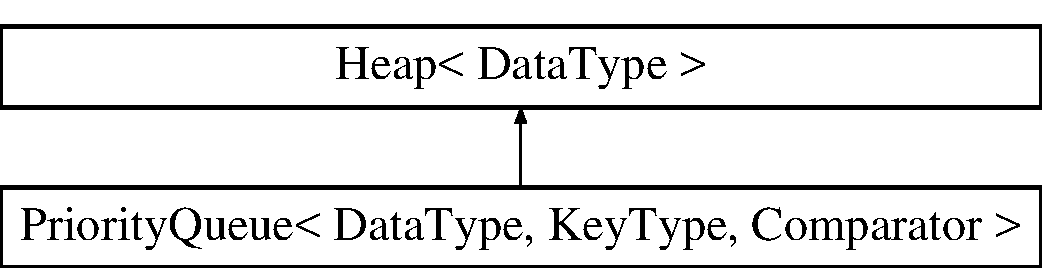
\includegraphics[height=2.000000cm]{class_priority_queue}
\end{center}
\end{figure}
\subsection*{Public Member Functions}
\begin{DoxyCompactItemize}
\item 
\hyperlink{class_priority_queue_a47de2a46cff1d6a6ed30a99c94dc1b14}{Priority\+Queue} (int max\+Number=\hyperlink{_priority_queue_8h_a88703212007be018800be64f2f5fde2f}{def\+Max\+Queue\+Size})
\begin{DoxyCompactList}\small\item\em The default constructor for the \hyperlink{class_priority_queue}{Priority\+Queue}. \end{DoxyCompactList}\item 
void \hyperlink{class_priority_queue_a61f3339cf0e87c67ed004f8eff0a1bfa}{enqueue} (const Data\+Type \&new\+Data\+Item)
\begin{DoxyCompactList}\small\item\em enqueue function for the Priorty\+Queue, it calls the insert function within the \hyperlink{class_heap}{Heap} A\+DT \end{DoxyCompactList}\item 
Data\+Type \hyperlink{class_priority_queue_a5bc758e313d6244e672ea6e81d695a46}{dequeue} ()
\begin{DoxyCompactList}\small\item\em dequeue function for the Priorty\+Queue, it calls the remove function within the \hyperlink{class_heap}{Heap} A\+DT \end{DoxyCompactList}\end{DoxyCompactItemize}
\subsection*{Additional Inherited Members}


\subsection{Constructor \& Destructor Documentation}
\index{Priority\+Queue@{Priority\+Queue}!Priority\+Queue@{Priority\+Queue}}
\index{Priority\+Queue@{Priority\+Queue}!Priority\+Queue@{Priority\+Queue}}
\subsubsection[{\texorpdfstring{Priority\+Queue(int max\+Number=def\+Max\+Queue\+Size)}{PriorityQueue(int maxNumber=defMaxQueueSize)}}]{\setlength{\rightskip}{0pt plus 5cm}template$<$typename Data\+Type , typename Key\+Type , typename Comparator $>$ {\bf Priority\+Queue}$<$ Data\+Type, Key\+Type, Comparator $>$\+::{\bf Priority\+Queue} (
\begin{DoxyParamCaption}
\item[{int}]{max\+Number = {\ttfamily {\bf def\+Max\+Queue\+Size}}}
\end{DoxyParamCaption}
)}\hypertarget{class_priority_queue_a47de2a46cff1d6a6ed30a99c94dc1b14}{}\label{class_priority_queue_a47de2a46cff1d6a6ed30a99c94dc1b14}


The default constructor for the \hyperlink{class_priority_queue}{Priority\+Queue}. 


\begin{DoxyParams}{Parameters}
{\em int} & max\+Number \\
\hline
\end{DoxyParams}
\begin{DoxyReturn}{Returns}
none 
\end{DoxyReturn}


\subsection{Member Function Documentation}
\index{Priority\+Queue@{Priority\+Queue}!dequeue@{dequeue}}
\index{dequeue@{dequeue}!Priority\+Queue@{Priority\+Queue}}
\subsubsection[{\texorpdfstring{dequeue()}{dequeue()}}]{\setlength{\rightskip}{0pt plus 5cm}template$<$typename Data\+Type , typename Key\+Type , typename Comparator $>$ Data\+Type {\bf Priority\+Queue}$<$ Data\+Type, Key\+Type, Comparator $>$\+::dequeue (
\begin{DoxyParamCaption}
{}
\end{DoxyParamCaption}
)}\hypertarget{class_priority_queue_a5bc758e313d6244e672ea6e81d695a46}{}\label{class_priority_queue_a5bc758e313d6244e672ea6e81d695a46}


dequeue function for the Priorty\+Queue, it calls the remove function within the \hyperlink{class_heap}{Heap} A\+DT 


\begin{DoxyParams}{Parameters}
{\em none} & \\
\hline
\end{DoxyParams}
\begin{DoxyReturn}{Returns}
none 
\end{DoxyReturn}
\index{Priority\+Queue@{Priority\+Queue}!enqueue@{enqueue}}
\index{enqueue@{enqueue}!Priority\+Queue@{Priority\+Queue}}
\subsubsection[{\texorpdfstring{enqueue(const Data\+Type \&new\+Data\+Item)}{enqueue(const DataType &newDataItem)}}]{\setlength{\rightskip}{0pt plus 5cm}template$<$typename Data\+Type , typename Key\+Type , typename Comparator $>$ void {\bf Priority\+Queue}$<$ Data\+Type, Key\+Type, Comparator $>$\+::enqueue (
\begin{DoxyParamCaption}
\item[{const Data\+Type \&}]{new\+Data\+Item}
\end{DoxyParamCaption}
)}\hypertarget{class_priority_queue_a61f3339cf0e87c67ed004f8eff0a1bfa}{}\label{class_priority_queue_a61f3339cf0e87c67ed004f8eff0a1bfa}


enqueue function for the Priorty\+Queue, it calls the insert function within the \hyperlink{class_heap}{Heap} A\+DT 


\begin{DoxyParams}{Parameters}
{\em const} & Data\+Type\& new\+Data\+Item \\
\hline
\end{DoxyParams}
\begin{DoxyReturn}{Returns}
none 
\end{DoxyReturn}


The documentation for this class was generated from the following files\+:\begin{DoxyCompactItemize}
\item 
\hyperlink{_priority_queue_8h}{Priority\+Queue.\+h}\item 
\hyperlink{_priority_queue_8cpp}{Priority\+Queue.\+cpp}\end{DoxyCompactItemize}

\hypertarget{struct_task_data}{}\section{Task\+Data Struct Reference}
\label{struct_task_data}\index{Task\+Data@{Task\+Data}}
\subsection*{Public Member Functions}
\begin{DoxyCompactItemize}
\item 
int \hyperlink{struct_task_data_a58cbe6eec8a86be7b827561a2f4b49c1}{get\+Priority} () const 
\item 
int \hyperlink{struct_task_data_a274a90c28f483fb7c8364c4e1441d8ff}{get\+Arrival} () const 
\end{DoxyCompactItemize}
\subsection*{Public Attributes}
\begin{DoxyCompactItemize}
\item 
int \hyperlink{struct_task_data_a9d8b606897eb428a62d816b71312e1b7}{priority}
\item 
int \hyperlink{struct_task_data_a126fafee3369b6a2d8734f4e46c670bc}{arrived}
\end{DoxyCompactItemize}


\subsection{Member Function Documentation}
\index{Task\+Data@{Task\+Data}!get\+Arrival@{get\+Arrival}}
\index{get\+Arrival@{get\+Arrival}!Task\+Data@{Task\+Data}}
\subsubsection[{\texorpdfstring{get\+Arrival() const }{getArrival() const }}]{\setlength{\rightskip}{0pt plus 5cm}int Task\+Data\+::get\+Arrival (
\begin{DoxyParamCaption}
{}
\end{DoxyParamCaption}
) const\hspace{0.3cm}{\ttfamily [inline]}}\hypertarget{struct_task_data_a274a90c28f483fb7c8364c4e1441d8ff}{}\label{struct_task_data_a274a90c28f483fb7c8364c4e1441d8ff}
\index{Task\+Data@{Task\+Data}!get\+Priority@{get\+Priority}}
\index{get\+Priority@{get\+Priority}!Task\+Data@{Task\+Data}}
\subsubsection[{\texorpdfstring{get\+Priority() const }{getPriority() const }}]{\setlength{\rightskip}{0pt plus 5cm}int Task\+Data\+::get\+Priority (
\begin{DoxyParamCaption}
{}
\end{DoxyParamCaption}
) const\hspace{0.3cm}{\ttfamily [inline]}}\hypertarget{struct_task_data_a58cbe6eec8a86be7b827561a2f4b49c1}{}\label{struct_task_data_a58cbe6eec8a86be7b827561a2f4b49c1}


\subsection{Member Data Documentation}
\index{Task\+Data@{Task\+Data}!arrived@{arrived}}
\index{arrived@{arrived}!Task\+Data@{Task\+Data}}
\subsubsection[{\texorpdfstring{arrived}{arrived}}]{\setlength{\rightskip}{0pt plus 5cm}int Task\+Data\+::arrived}\hypertarget{struct_task_data_a126fafee3369b6a2d8734f4e46c670bc}{}\label{struct_task_data_a126fafee3369b6a2d8734f4e46c670bc}
\index{Task\+Data@{Task\+Data}!priority@{priority}}
\index{priority@{priority}!Task\+Data@{Task\+Data}}
\subsubsection[{\texorpdfstring{priority}{priority}}]{\setlength{\rightskip}{0pt plus 5cm}int Task\+Data\+::priority}\hypertarget{struct_task_data_a9d8b606897eb428a62d816b71312e1b7}{}\label{struct_task_data_a9d8b606897eb428a62d816b71312e1b7}


The documentation for this struct was generated from the following file\+:\begin{DoxyCompactItemize}
\item 
\hyperlink{ossim_8cpp}{ossim.\+cpp}\end{DoxyCompactItemize}

\hypertarget{class_test_data}{}\section{Test\+Data Class Reference}
\label{class_test_data}\index{Test\+Data@{Test\+Data}}
\subsection*{Public Member Functions}
\begin{DoxyCompactItemize}
\item 
void \hyperlink{class_test_data_af6c76355a3ab75cd07ca6bba7dfe2115}{set\+Priority} (int new\+Priority)
\item 
int \hyperlink{class_test_data_a11f3f060f167d1989c94bf94860aed20}{get\+Priority} () const 
\item 
void \hyperlink{class_test_data_af6c76355a3ab75cd07ca6bba7dfe2115}{set\+Priority} (int new\+Priority)
\item 
int \hyperlink{class_test_data_a11f3f060f167d1989c94bf94860aed20}{get\+Priority} () const 
\end{DoxyCompactItemize}


\subsection{Member Function Documentation}
\index{Test\+Data@{Test\+Data}!get\+Priority@{get\+Priority}}
\index{get\+Priority@{get\+Priority}!Test\+Data@{Test\+Data}}
\subsubsection[{\texorpdfstring{get\+Priority() const }{getPriority() const }}]{\setlength{\rightskip}{0pt plus 5cm}int Test\+Data\+::get\+Priority (
\begin{DoxyParamCaption}
{}
\end{DoxyParamCaption}
) const\hspace{0.3cm}{\ttfamily [inline]}}\hypertarget{class_test_data_a11f3f060f167d1989c94bf94860aed20}{}\label{class_test_data_a11f3f060f167d1989c94bf94860aed20}
\index{Test\+Data@{Test\+Data}!get\+Priority@{get\+Priority}}
\index{get\+Priority@{get\+Priority}!Test\+Data@{Test\+Data}}
\subsubsection[{\texorpdfstring{get\+Priority() const }{getPriority() const }}]{\setlength{\rightskip}{0pt plus 5cm}int Test\+Data\+::get\+Priority (
\begin{DoxyParamCaption}
{}
\end{DoxyParamCaption}
) const\hspace{0.3cm}{\ttfamily [inline]}}\hypertarget{class_test_data_a11f3f060f167d1989c94bf94860aed20}{}\label{class_test_data_a11f3f060f167d1989c94bf94860aed20}
\index{Test\+Data@{Test\+Data}!set\+Priority@{set\+Priority}}
\index{set\+Priority@{set\+Priority}!Test\+Data@{Test\+Data}}
\subsubsection[{\texorpdfstring{set\+Priority(int new\+Priority)}{setPriority(int newPriority)}}]{\setlength{\rightskip}{0pt plus 5cm}void Test\+Data\+::set\+Priority (
\begin{DoxyParamCaption}
\item[{int}]{new\+Priority}
\end{DoxyParamCaption}
)\hspace{0.3cm}{\ttfamily [inline]}}\hypertarget{class_test_data_af6c76355a3ab75cd07ca6bba7dfe2115}{}\label{class_test_data_af6c76355a3ab75cd07ca6bba7dfe2115}
\index{Test\+Data@{Test\+Data}!set\+Priority@{set\+Priority}}
\index{set\+Priority@{set\+Priority}!Test\+Data@{Test\+Data}}
\subsubsection[{\texorpdfstring{set\+Priority(int new\+Priority)}{setPriority(int newPriority)}}]{\setlength{\rightskip}{0pt plus 5cm}void Test\+Data\+::set\+Priority (
\begin{DoxyParamCaption}
\item[{int}]{new\+Priority}
\end{DoxyParamCaption}
)\hspace{0.3cm}{\ttfamily [inline]}}\hypertarget{class_test_data_af6c76355a3ab75cd07ca6bba7dfe2115}{}\label{class_test_data_af6c76355a3ab75cd07ca6bba7dfe2115}


The documentation for this class was generated from the following files\+:\begin{DoxyCompactItemize}
\item 
\hyperlink{test11hs_8cpp}{test11hs.\+cpp}\item 
\hyperlink{test11pq_8cpp}{test11pq.\+cpp}\end{DoxyCompactItemize}

\hypertarget{class_test_data_item}{}\section{Test\+Data\+Item$<$ Key\+Type $>$ Class Template Reference}
\label{class_test_data_item}\index{Test\+Data\+Item$<$ Key\+Type $>$@{Test\+Data\+Item$<$ Key\+Type $>$}}
\subsection*{Public Member Functions}
\begin{DoxyCompactItemize}
\item 
\hyperlink{class_test_data_item_adfbd4f5d142caf3d95c96940f96c1d85}{Test\+Data\+Item} ()
\item 
void \hyperlink{class_test_data_item_a84667429c081b1dbb212956c88011216}{set\+Priority} (Key\+Type new\+Pty)
\item 
Key\+Type \hyperlink{class_test_data_item_ac1632213d959555ec8f5aee8a1505d72}{get\+Priority} () const 
\item 
\hyperlink{class_test_data_item}{Test\+Data\+Item} \& \hyperlink{class_test_data_item_aa77cd6be3773b0767182c22644ae4490}{operator=} (const \hyperlink{class_test_data_item}{Test\+Data\+Item} \&orig)
\end{DoxyCompactItemize}


\subsection{Constructor \& Destructor Documentation}
\index{Test\+Data\+Item@{Test\+Data\+Item}!Test\+Data\+Item@{Test\+Data\+Item}}
\index{Test\+Data\+Item@{Test\+Data\+Item}!Test\+Data\+Item@{Test\+Data\+Item}}
\subsubsection[{\texorpdfstring{Test\+Data\+Item()}{TestDataItem()}}]{\setlength{\rightskip}{0pt plus 5cm}template$<$typename Key\+Type $>$ {\bf Test\+Data\+Item}$<$ Key\+Type $>$\+::{\bf Test\+Data\+Item} (
\begin{DoxyParamCaption}
{}
\end{DoxyParamCaption}
)\hspace{0.3cm}{\ttfamily [inline]}}\hypertarget{class_test_data_item_adfbd4f5d142caf3d95c96940f96c1d85}{}\label{class_test_data_item_adfbd4f5d142caf3d95c96940f96c1d85}


\subsection{Member Function Documentation}
\index{Test\+Data\+Item@{Test\+Data\+Item}!get\+Priority@{get\+Priority}}
\index{get\+Priority@{get\+Priority}!Test\+Data\+Item@{Test\+Data\+Item}}
\subsubsection[{\texorpdfstring{get\+Priority() const }{getPriority() const }}]{\setlength{\rightskip}{0pt plus 5cm}template$<$typename Key\+Type $>$ Key\+Type {\bf Test\+Data\+Item}$<$ Key\+Type $>$\+::get\+Priority (
\begin{DoxyParamCaption}
{}
\end{DoxyParamCaption}
) const\hspace{0.3cm}{\ttfamily [inline]}}\hypertarget{class_test_data_item_ac1632213d959555ec8f5aee8a1505d72}{}\label{class_test_data_item_ac1632213d959555ec8f5aee8a1505d72}
\index{Test\+Data\+Item@{Test\+Data\+Item}!operator=@{operator=}}
\index{operator=@{operator=}!Test\+Data\+Item@{Test\+Data\+Item}}
\subsubsection[{\texorpdfstring{operator=(const Test\+Data\+Item \&orig)}{operator=(const TestDataItem &orig)}}]{\setlength{\rightskip}{0pt plus 5cm}template$<$typename Key\+Type $>$ {\bf Test\+Data\+Item}\& {\bf Test\+Data\+Item}$<$ Key\+Type $>$\+::operator= (
\begin{DoxyParamCaption}
\item[{const {\bf Test\+Data\+Item}$<$ Key\+Type $>$ \&}]{orig}
\end{DoxyParamCaption}
)\hspace{0.3cm}{\ttfamily [inline]}}\hypertarget{class_test_data_item_aa77cd6be3773b0767182c22644ae4490}{}\label{class_test_data_item_aa77cd6be3773b0767182c22644ae4490}
\index{Test\+Data\+Item@{Test\+Data\+Item}!set\+Priority@{set\+Priority}}
\index{set\+Priority@{set\+Priority}!Test\+Data\+Item@{Test\+Data\+Item}}
\subsubsection[{\texorpdfstring{set\+Priority(\+Key\+Type new\+Pty)}{setPriority(KeyType newPty)}}]{\setlength{\rightskip}{0pt plus 5cm}template$<$typename Key\+Type $>$ void {\bf Test\+Data\+Item}$<$ Key\+Type $>$\+::set\+Priority (
\begin{DoxyParamCaption}
\item[{Key\+Type}]{new\+Pty}
\end{DoxyParamCaption}
)\hspace{0.3cm}{\ttfamily [inline]}}\hypertarget{class_test_data_item_a84667429c081b1dbb212956c88011216}{}\label{class_test_data_item_a84667429c081b1dbb212956c88011216}


The documentation for this class was generated from the following file\+:\begin{DoxyCompactItemize}
\item 
\hyperlink{test11_8cpp}{test11.\+cpp}\end{DoxyCompactItemize}

\chapter{File Documentation}
\hypertarget{config_8h}{}\section{config.\+h File Reference}
\label{config_8h}\index{config.\+h@{config.\+h}}
\subsection*{Macros}
\begin{DoxyCompactItemize}
\item 
\#define \hyperlink{config_8h_a37256be1bc236d447e0bfb4668d06e08}{L\+A\+B12\+\_\+\+T\+E\+S\+T1}~1
\item 
\#define \hyperlink{config_8h_a4e475097daefad258dd91becac6afa97}{L\+A\+B12\+\_\+\+T\+E\+S\+T2}~0
\item 
\#define \hyperlink{config_8h_a0796ef74cc24d4f0e3eeb82b48dc8d3e}{L\+A\+B12\+\_\+\+T\+E\+S\+T3}~1
\end{DoxyCompactItemize}


\subsection{Macro Definition Documentation}
\index{config.\+h@{config.\+h}!L\+A\+B12\+\_\+\+T\+E\+S\+T1@{L\+A\+B12\+\_\+\+T\+E\+S\+T1}}
\index{L\+A\+B12\+\_\+\+T\+E\+S\+T1@{L\+A\+B12\+\_\+\+T\+E\+S\+T1}!config.\+h@{config.\+h}}
\subsubsection[{\texorpdfstring{L\+A\+B12\+\_\+\+T\+E\+S\+T1}{LAB12_TEST1}}]{\setlength{\rightskip}{0pt plus 5cm}\#define L\+A\+B12\+\_\+\+T\+E\+S\+T1~1}\hypertarget{config_8h_a37256be1bc236d447e0bfb4668d06e08}{}\label{config_8h_a37256be1bc236d447e0bfb4668d06e08}
\hyperlink{class_weighted_graph}{Weighted\+Graph} class configuration file. Activate test \#N by defining the corresponding L\+A\+B12\+\_\+\+T\+E\+S\+TN to have the value 1. \index{config.\+h@{config.\+h}!L\+A\+B12\+\_\+\+T\+E\+S\+T2@{L\+A\+B12\+\_\+\+T\+E\+S\+T2}}
\index{L\+A\+B12\+\_\+\+T\+E\+S\+T2@{L\+A\+B12\+\_\+\+T\+E\+S\+T2}!config.\+h@{config.\+h}}
\subsubsection[{\texorpdfstring{L\+A\+B12\+\_\+\+T\+E\+S\+T2}{LAB12_TEST2}}]{\setlength{\rightskip}{0pt plus 5cm}\#define L\+A\+B12\+\_\+\+T\+E\+S\+T2~0}\hypertarget{config_8h_a4e475097daefad258dd91becac6afa97}{}\label{config_8h_a4e475097daefad258dd91becac6afa97}
\index{config.\+h@{config.\+h}!L\+A\+B12\+\_\+\+T\+E\+S\+T3@{L\+A\+B12\+\_\+\+T\+E\+S\+T3}}
\index{L\+A\+B12\+\_\+\+T\+E\+S\+T3@{L\+A\+B12\+\_\+\+T\+E\+S\+T3}!config.\+h@{config.\+h}}
\subsubsection[{\texorpdfstring{L\+A\+B12\+\_\+\+T\+E\+S\+T3}{LAB12_TEST3}}]{\setlength{\rightskip}{0pt plus 5cm}\#define L\+A\+B12\+\_\+\+T\+E\+S\+T3~1}\hypertarget{config_8h_a0796ef74cc24d4f0e3eeb82b48dc8d3e}{}\label{config_8h_a0796ef74cc24d4f0e3eeb82b48dc8d3e}

\hypertarget{_heap_8cpp}{}\section{Heap.\+cpp File Reference}
\label{_heap_8cpp}\index{Heap.\+cpp@{Heap.\+cpp}}


An implementation file for a \hyperlink{class_heap}{Heap}.  


{\ttfamily \#include \char`\"{}Heap.\+h\char`\"{}}\\*
{\ttfamily \#include \char`\"{}show11.\+cpp\char`\"{}}\\*


\subsection{Detailed Description}
An implementation file for a \hyperlink{class_heap}{Heap}. 

\begin{DoxyAuthor}{Author}
Christopher Eichstedt 
\end{DoxyAuthor}

\hypertarget{_heap_8h}{}\section{Heap.\+h File Reference}
\label{_heap_8h}\index{Heap.\+h@{Heap.\+h}}
{\ttfamily \#include $<$stdexcept$>$}\\*
{\ttfamily \#include $<$iostream$>$}\\*
\subsection*{Classes}
\begin{DoxyCompactItemize}
\item 
class \hyperlink{class_less}{Less$<$ Key\+Type $>$}
\item 
class \hyperlink{class_heap}{Heap$<$ Data\+Type, Key\+Type, Comparator $>$}
\end{DoxyCompactItemize}

\hypertarget{heapsort_8cs}{}\section{heapsort.\+cs File Reference}
\label{heapsort_8cs}\index{heapsort.\+cs@{heapsort.\+cs}}
\subsection*{Functions}
\begin{DoxyCompactItemize}
\item 
void \hyperlink{heapsort_8cs_ace0c151b0a221e24a1aad0bf9a821c2f}{move\+Down} (Data\+Type data\+Items\mbox{[}$\,$\mbox{]}, int root, int size)
\item 
void \hyperlink{heapsort_8cs_a1b9d07732ab0ab5fb1c3fabfb8ba4f4b}{heap\+Sort} (Data\+Type data\+Items\mbox{[}$\,$\mbox{]}, int size)
\end{DoxyCompactItemize}


\subsection{Function Documentation}
\index{heapsort.\+cs@{heapsort.\+cs}!heap\+Sort@{heap\+Sort}}
\index{heap\+Sort@{heap\+Sort}!heapsort.\+cs@{heapsort.\+cs}}
\subsubsection[{\texorpdfstring{heap\+Sort(\+Data\+Type data\+Items[], int size)}{heapSort(DataType dataItems[], int size)}}]{\setlength{\rightskip}{0pt plus 5cm}void heap\+Sort (
\begin{DoxyParamCaption}
\item[{Data\+Type}]{data\+Items\mbox{[}$\,$\mbox{]}, }
\item[{int}]{size}
\end{DoxyParamCaption}
)}\hypertarget{heapsort_8cs_a1b9d07732ab0ab5fb1c3fabfb8ba4f4b}{}\label{heapsort_8cs_a1b9d07732ab0ab5fb1c3fabfb8ba4f4b}
\index{heapsort.\+cs@{heapsort.\+cs}!move\+Down@{move\+Down}}
\index{move\+Down@{move\+Down}!heapsort.\+cs@{heapsort.\+cs}}
\subsubsection[{\texorpdfstring{move\+Down(\+Data\+Type data\+Items[], int root, int size)}{moveDown(DataType dataItems[], int root, int size)}}]{\setlength{\rightskip}{0pt plus 5cm}void move\+Down (
\begin{DoxyParamCaption}
\item[{Data\+Type}]{data\+Items\mbox{[}$\,$\mbox{]}, }
\item[{int}]{root, }
\item[{int}]{size}
\end{DoxyParamCaption}
)}\hypertarget{heapsort_8cs_ace0c151b0a221e24a1aad0bf9a821c2f}{}\label{heapsort_8cs_ace0c151b0a221e24a1aad0bf9a821c2f}

\hypertarget{ossim_8cpp}{}\section{ossim.\+cpp File Reference}
\label{ossim_8cpp}\index{ossim.\+cpp@{ossim.\+cpp}}
{\ttfamily \#include $<$iostream$>$}\\*
{\ttfamily \#include $<$cstdlib$>$}\\*
{\ttfamily \#include \char`\"{}Priority\+Queue.\+cpp\char`\"{}}\\*
\subsection*{Classes}
\begin{DoxyCompactItemize}
\item 
struct \hyperlink{struct_task_data}{Task\+Data}
\end{DoxyCompactItemize}
\subsection*{Functions}
\begin{DoxyCompactItemize}
\item 
int \hyperlink{ossim_8cpp_ae66f6b31b5ad750f1fe042a706a4e3d4}{main} ()
\end{DoxyCompactItemize}


\subsection{Function Documentation}
\index{ossim.\+cpp@{ossim.\+cpp}!main@{main}}
\index{main@{main}!ossim.\+cpp@{ossim.\+cpp}}
\subsubsection[{\texorpdfstring{main()}{main()}}]{\setlength{\rightskip}{0pt plus 5cm}int main (
\begin{DoxyParamCaption}
{}
\end{DoxyParamCaption}
)}\hypertarget{ossim_8cpp_ae66f6b31b5ad750f1fe042a706a4e3d4}{}\label{ossim_8cpp_ae66f6b31b5ad750f1fe042a706a4e3d4}

\hypertarget{_priority_queue_8cpp}{}\section{Priority\+Queue.\+cpp File Reference}
\label{_priority_queue_8cpp}\index{Priority\+Queue.\+cpp@{Priority\+Queue.\+cpp}}


An implementation file for a Priorty Queue.  


{\ttfamily \#include \char`\"{}Priority\+Queue.\+h\char`\"{}}\\*


\subsection{Detailed Description}
An implementation file for a Priorty Queue. 

\begin{DoxyAuthor}{Author}
Christopher Eichstedt 
\end{DoxyAuthor}

\hypertarget{_priority_queue_8h}{}\section{Priority\+Queue.\+h File Reference}
\label{_priority_queue_8h}\index{Priority\+Queue.\+h@{Priority\+Queue.\+h}}
{\ttfamily \#include $<$stdexcept$>$}\\*
{\ttfamily \#include $<$iostream$>$}\\*
{\ttfamily \#include \char`\"{}Heap.\+cpp\char`\"{}}\\*
\subsection*{Classes}
\begin{DoxyCompactItemize}
\item 
class \hyperlink{class_priority_queue}{Priority\+Queue$<$ Data\+Type, Key\+Type, Comparator $>$}
\end{DoxyCompactItemize}
\subsection*{Variables}
\begin{DoxyCompactItemize}
\item 
const int \hyperlink{_priority_queue_8h_a88703212007be018800be64f2f5fde2f}{def\+Max\+Queue\+Size} = 10
\end{DoxyCompactItemize}


\subsection{Variable Documentation}
\index{Priority\+Queue.\+h@{Priority\+Queue.\+h}!def\+Max\+Queue\+Size@{def\+Max\+Queue\+Size}}
\index{def\+Max\+Queue\+Size@{def\+Max\+Queue\+Size}!Priority\+Queue.\+h@{Priority\+Queue.\+h}}
\subsubsection[{\texorpdfstring{def\+Max\+Queue\+Size}{defMaxQueueSize}}]{\setlength{\rightskip}{0pt plus 5cm}const int def\+Max\+Queue\+Size = 10}\hypertarget{_priority_queue_8h_a88703212007be018800be64f2f5fde2f}{}\label{_priority_queue_8h_a88703212007be018800be64f2f5fde2f}

\hypertarget{show11_8cpp}{}\section{show11.\+cpp File Reference}
\label{show11_8cpp}\index{show11.\+cpp@{show11.\+cpp}}

\hypertarget{test11_8cpp}{}\section{test11.\+cpp File Reference}
\label{test11_8cpp}\index{test11.\+cpp@{test11.\+cpp}}
{\ttfamily \#include $<$iostream$>$}\\*
{\ttfamily \#include $<$string$>$}\\*
{\ttfamily \#include $<$cctype$>$}\\*
{\ttfamily \#include \char`\"{}Heap.\+cpp\char`\"{}}\\*
{\ttfamily \#include \char`\"{}config.\+h\char`\"{}}\\*
\subsection*{Classes}
\begin{DoxyCompactItemize}
\item 
class \hyperlink{class_test_data_item}{Test\+Data\+Item$<$ Key\+Type $>$}
\item 
class \hyperlink{class_greater}{Greater$<$ Key\+Type $>$}
\end{DoxyCompactItemize}
\subsection*{Functions}
\begin{DoxyCompactItemize}
\item 
void \hyperlink{test11_8cpp_a0d20b69b0ad703df78459e1033d5c1d4}{print\+Help} ()
\item 
int \hyperlink{test11_8cpp_ae66f6b31b5ad750f1fe042a706a4e3d4}{main} ()
\end{DoxyCompactItemize}


\subsection{Function Documentation}
\index{test11.\+cpp@{test11.\+cpp}!main@{main}}
\index{main@{main}!test11.\+cpp@{test11.\+cpp}}
\subsubsection[{\texorpdfstring{main()}{main()}}]{\setlength{\rightskip}{0pt plus 5cm}int main (
\begin{DoxyParamCaption}
{}
\end{DoxyParamCaption}
)}\hypertarget{test11_8cpp_ae66f6b31b5ad750f1fe042a706a4e3d4}{}\label{test11_8cpp_ae66f6b31b5ad750f1fe042a706a4e3d4}
\index{test11.\+cpp@{test11.\+cpp}!print\+Help@{print\+Help}}
\index{print\+Help@{print\+Help}!test11.\+cpp@{test11.\+cpp}}
\subsubsection[{\texorpdfstring{print\+Help()}{printHelp()}}]{\setlength{\rightskip}{0pt plus 5cm}void print\+Help (
\begin{DoxyParamCaption}
{}
\end{DoxyParamCaption}
)}\hypertarget{test11_8cpp_a0d20b69b0ad703df78459e1033d5c1d4}{}\label{test11_8cpp_a0d20b69b0ad703df78459e1033d5c1d4}

\hypertarget{test11hs_8cpp}{}\section{test11hs.\+cpp File Reference}
\label{test11hs_8cpp}\index{test11hs.\+cpp@{test11hs.\+cpp}}
{\ttfamily \#include $<$iostream$>$}\\*
{\ttfamily \#include \char`\"{}heapsort.\+cpp\char`\"{}}\\*
\subsection*{Classes}
\begin{DoxyCompactItemize}
\item 
class \hyperlink{class_test_data}{Test\+Data}
\end{DoxyCompactItemize}
\subsection*{Functions}
\begin{DoxyCompactItemize}
\item 
int \hyperlink{test11hs_8cpp_ae66f6b31b5ad750f1fe042a706a4e3d4}{main} ()
\end{DoxyCompactItemize}
\subsection*{Variables}
\begin{DoxyCompactItemize}
\item 
const int \hyperlink{test11hs_8cpp_af9ecea2a656a85cc42eb181a9976ad31}{M\+A\+X\+\_\+\+N\+U\+M\+\_\+\+D\+A\+T\+A\+\_\+\+I\+T\+E\+MS} = 10
\end{DoxyCompactItemize}


\subsection{Function Documentation}
\index{test11hs.\+cpp@{test11hs.\+cpp}!main@{main}}
\index{main@{main}!test11hs.\+cpp@{test11hs.\+cpp}}
\subsubsection[{\texorpdfstring{main()}{main()}}]{\setlength{\rightskip}{0pt plus 5cm}int main (
\begin{DoxyParamCaption}
{}
\end{DoxyParamCaption}
)}\hypertarget{test11hs_8cpp_ae66f6b31b5ad750f1fe042a706a4e3d4}{}\label{test11hs_8cpp_ae66f6b31b5ad750f1fe042a706a4e3d4}


\subsection{Variable Documentation}
\index{test11hs.\+cpp@{test11hs.\+cpp}!M\+A\+X\+\_\+\+N\+U\+M\+\_\+\+D\+A\+T\+A\+\_\+\+I\+T\+E\+MS@{M\+A\+X\+\_\+\+N\+U\+M\+\_\+\+D\+A\+T\+A\+\_\+\+I\+T\+E\+MS}}
\index{M\+A\+X\+\_\+\+N\+U\+M\+\_\+\+D\+A\+T\+A\+\_\+\+I\+T\+E\+MS@{M\+A\+X\+\_\+\+N\+U\+M\+\_\+\+D\+A\+T\+A\+\_\+\+I\+T\+E\+MS}!test11hs.\+cpp@{test11hs.\+cpp}}
\subsubsection[{\texorpdfstring{M\+A\+X\+\_\+\+N\+U\+M\+\_\+\+D\+A\+T\+A\+\_\+\+I\+T\+E\+MS}{MAX_NUM_DATA_ITEMS}}]{\setlength{\rightskip}{0pt plus 5cm}const int M\+A\+X\+\_\+\+N\+U\+M\+\_\+\+D\+A\+T\+A\+\_\+\+I\+T\+E\+MS = 10}\hypertarget{test11hs_8cpp_af9ecea2a656a85cc42eb181a9976ad31}{}\label{test11hs_8cpp_af9ecea2a656a85cc42eb181a9976ad31}

\hypertarget{test11pq_8cpp}{}\section{test11pq.\+cpp File Reference}
\label{test11pq_8cpp}\index{test11pq.\+cpp@{test11pq.\+cpp}}
{\ttfamily \#include $<$iostream$>$}\\*
{\ttfamily \#include $<$cctype$>$}\\*
{\ttfamily \#include \char`\"{}Priority\+Queue.\+cpp\char`\"{}}\\*
\subsection*{Classes}
\begin{DoxyCompactItemize}
\item 
class \hyperlink{class_test_data}{Test\+Data}
\end{DoxyCompactItemize}
\subsection*{Functions}
\begin{DoxyCompactItemize}
\item 
void \hyperlink{test11pq_8cpp_a0d20b69b0ad703df78459e1033d5c1d4}{print\+Help} ()
\item 
int \hyperlink{test11pq_8cpp_ae66f6b31b5ad750f1fe042a706a4e3d4}{main} ()
\end{DoxyCompactItemize}


\subsection{Function Documentation}
\index{test11pq.\+cpp@{test11pq.\+cpp}!main@{main}}
\index{main@{main}!test11pq.\+cpp@{test11pq.\+cpp}}
\subsubsection[{\texorpdfstring{main()}{main()}}]{\setlength{\rightskip}{0pt plus 5cm}int main (
\begin{DoxyParamCaption}
{}
\end{DoxyParamCaption}
)}\hypertarget{test11pq_8cpp_ae66f6b31b5ad750f1fe042a706a4e3d4}{}\label{test11pq_8cpp_ae66f6b31b5ad750f1fe042a706a4e3d4}
\index{test11pq.\+cpp@{test11pq.\+cpp}!print\+Help@{print\+Help}}
\index{print\+Help@{print\+Help}!test11pq.\+cpp@{test11pq.\+cpp}}
\subsubsection[{\texorpdfstring{print\+Help()}{printHelp()}}]{\setlength{\rightskip}{0pt plus 5cm}void print\+Help (
\begin{DoxyParamCaption}
{}
\end{DoxyParamCaption}
)}\hypertarget{test11pq_8cpp_a0d20b69b0ad703df78459e1033d5c1d4}{}\label{test11pq_8cpp_a0d20b69b0ad703df78459e1033d5c1d4}

%--- End generated contents ---

% Index
\backmatter
\newpage
\phantomsection
\clearemptydoublepage
\addcontentsline{toc}{chapter}{Index}
\printindex

\end{document}
